\documentclass{article}

% Language setting
% Replace `english' with e.g. `spanish' to change the document language
\usepackage[english]{babel}
\usepackage{caption}
% Set page size and margins
% Replace `letterpaper' with`a4paper' for UK/EU standard size
\usepackage[letterpaper,top=2cm,bottom=2cm,left=3cm,right=3cm,marginparwidth=1.75cm]{geometry}

% Useful packages
\usepackage{amsmath}
\usepackage{graphicx}
\usepackage{authblk} % this is for multiple authors 
\usepackage[colorlinks=true, allcolors=blue]{hyperref}
\usepackage{cleveref}

% Configure for "Fig.":
\crefname{figure}{Fig.}{Figs.}
\Crefname{figure}{Fig.}{Figs.}


% reference configuration
\usepackage[authoryear,round]{natbib}
\bibliographystyle{apalike} % for an APA-like style

%%%%%%%%%%%%%%%%%%%%%%%%%%%%%%%%%%%%
%%% --- Tittle of the paper --- %%%
%%%%%%%%%%%%%%%%%%%%%%%%%%%%%%%%%%
\title{Suppementary materials: Development of outdoor air pollution models for estimating exposure in the Barcelona Life Study Cohort (BiSC)}

%%%%%%%%%%%%%%%%%%%%%%%%%%%%%%%%%%%%%%%%%
%%% --- Authors and affiliations --- %%%
%%%%%%%%%%%%%%%%%%%%%%%%%%%%%%%%%%%%%%%

%%% --- Authors --- %%%
\author[1, 2]{Alan Domínguez}
\author[1]{Marta Cirach}
\author[1,3]{Ioar Rivas}
\author[1]{Bruno Raimbault}
\author[1]{Toni Galmes}
\author[1,2,3]{Jordi Sunyer}
\author[1, 3, 4]{Payam Dadvand}
\author[1,2,3]{Xavier Basagaña}

%%% --- Affiliations --- %%%
\affil[1]{Barcelona Institute for Global Health (ISGlobal), Barcelona, Spain.}
\affil[2]{Universitat Popmpeu Fabra (UPF), Barcelona, Spain.}
\affil[3]{CIBER Epidemiología y Salud Pública (CIBERESP), Madrid, Spain.}
\affil[4]{London School of Hygiene and Tropical Medicine ( LSHTM), London, UK.}

%%%%%%%%%%%%%%%%%%%%%%%%%%%%%%%%%%%%%%%%%%%%%%%%%%%%%%%%%%%%%%%%%%%%%%%%%

\begin{document}
\maketitle

\section{Introduction}

Air pollution stands as the primary environmental risk factor for human health \cite{} and plays a significant role in the global burden of disease \cite{}. Exposure to ambient air pollution has been linked with a extensive array of adverse health outcomes\cite{}. Urbanization has played a pivotal in this context, increasing air pollution exposure as cities grow and more population moves to urban areas\cite{}. This trend presents challenges for epidemiological studies, where accurate estimates capturing both the spatial and temporal variability are essential to evaluate the short- and long-term health impacts of air pollution\cite{}. Recent years have witnessed advancements in spatiotemporal modelling of air pollution across large-scale domains. While European-wide models 
aimed to assess long-term air pollution exposure effects, their ability to predict at micro-scales has been limited\cite{}. Therefore, a detailed and comprehensive assessment of air pollution exposure at smaller areas is essential for understanding its impact on health, especially during critical developmental phases\cite{}.

Over the past few decades, several modelling techniques have been adopted in environmental epidemiology to determine exposure concentrations of air pollution\cite{}. Among these, Land use regression (LUR) and dispersion models (DM) are the most common approaches for estimating air pollution exposure concentrations in cohort studies. LUR models employ regression techniques to predict air pollution levels at non-monitored locations, drawing on observed air pollution data and spatial explanatory variables that works as proxies for traffic related air pollution\cite{}. In contrast, DMs rely on mathematical simulations to estimate air pollution levels. These predictions are based on data from emissions sources, chemical transformations, pollutant dispersion, topography, roughness, and meteorological data\cite{}. In order to overcome the shortcomings of the aforementioned approaches, hybrid models (HM) have emerged recently, blending both spatial and temporal advantages, leading to refined and enhanced estimations\cite{}. These models combined outputs from dispersion, land use variables, and  data from monitoring station\cite{}.

Further complexity arise in urban areas when modelling air pollution, due to complex spatiotemporal patterns that difficult accurate estimation of ground-level air pollutant concentrations\cite{}. As a consequence, machine learning (ML) algorithms have been used, particularly decision trees based methods used due their ability to model non-linear and potential interaction among predictive variables \cite{}. Among the different ML algorithm, random forest has emerged as one of the most robust techniques for predicting air pollution concentrations\cite{}.

In this study, we developed spatiotemporal models using different methodologies (LUR, DM, and HM) to estimate outdoor air pollution exposure for specific air pollutants, all under the framework of the Barcelona Life Study Cohort (BiSC). While LUR and DM, will be built using conventional techniques, the HM will harness the Random Forest (RF) algorithm, integrating outputs from the DM and explanatory variables from the LUR model. The overall objective is to obtain accurate NO\textsubscript{2}, PM\textsubscript{2.5}, PM\textsubscript{2.5} constituents (Fe, Zn, Cu, Sb), and BC estimates for use in prenatal exposure assessment for the BiSC cohort study. 

%%%%%%%%%%%%%%%%%%%%%%%%%%%%%%%%%%%%
%%% --- Material and methods--- %%%%%%%%%%%%%%%%%%%%%%%%%%%%%%%%%%%%%
%%%%%%%%%%%%%%%%%%%%%%%%%%%%%%%%%%%
\section{Materials and methods}

%%%%%%%%%%%%%%%%%%%%%%%%%%%%%%%%%%%%%%%%%%%%%%%%%%%%%
%%% --- Study domain and Monitoring Campaigns --- %%%
%%%%%%%%%%%%%%%%%%%%%%%%%%%%%%%%%%%%%%%%%%%%%%%%%%%%
\subsection{Study domain and monitoring campaigns}

Barcelona (\textbf{\cref{fig1}}), is one of the most populated and dense cities in Spain, with 1,656,725 inhabitants ($\approx16,255.4$ inhabitants/km\textsuperscript{2}). It is located on the Mediterranean coast of the Iberian peninsula, protected by the Collserola mountain range and delimited by two delta rives (Besòs and LLobregat). The city has a Mediterranean climate, the wind patterns are dominated by a breeze that blows from the sea during the daytime and from the land during nigh-time. Barcelona is one of the cities in Europe with the highest vehicle traffic density (6,000 vehicles/km\textsuperscript{2}) \cite{casallas2018}. 

% Put the figure text closer to the Figure 1
\captionsetup[figure]{skip=-4pt}
% We add the figure with the study domain 
\begin{figure}[!htb]
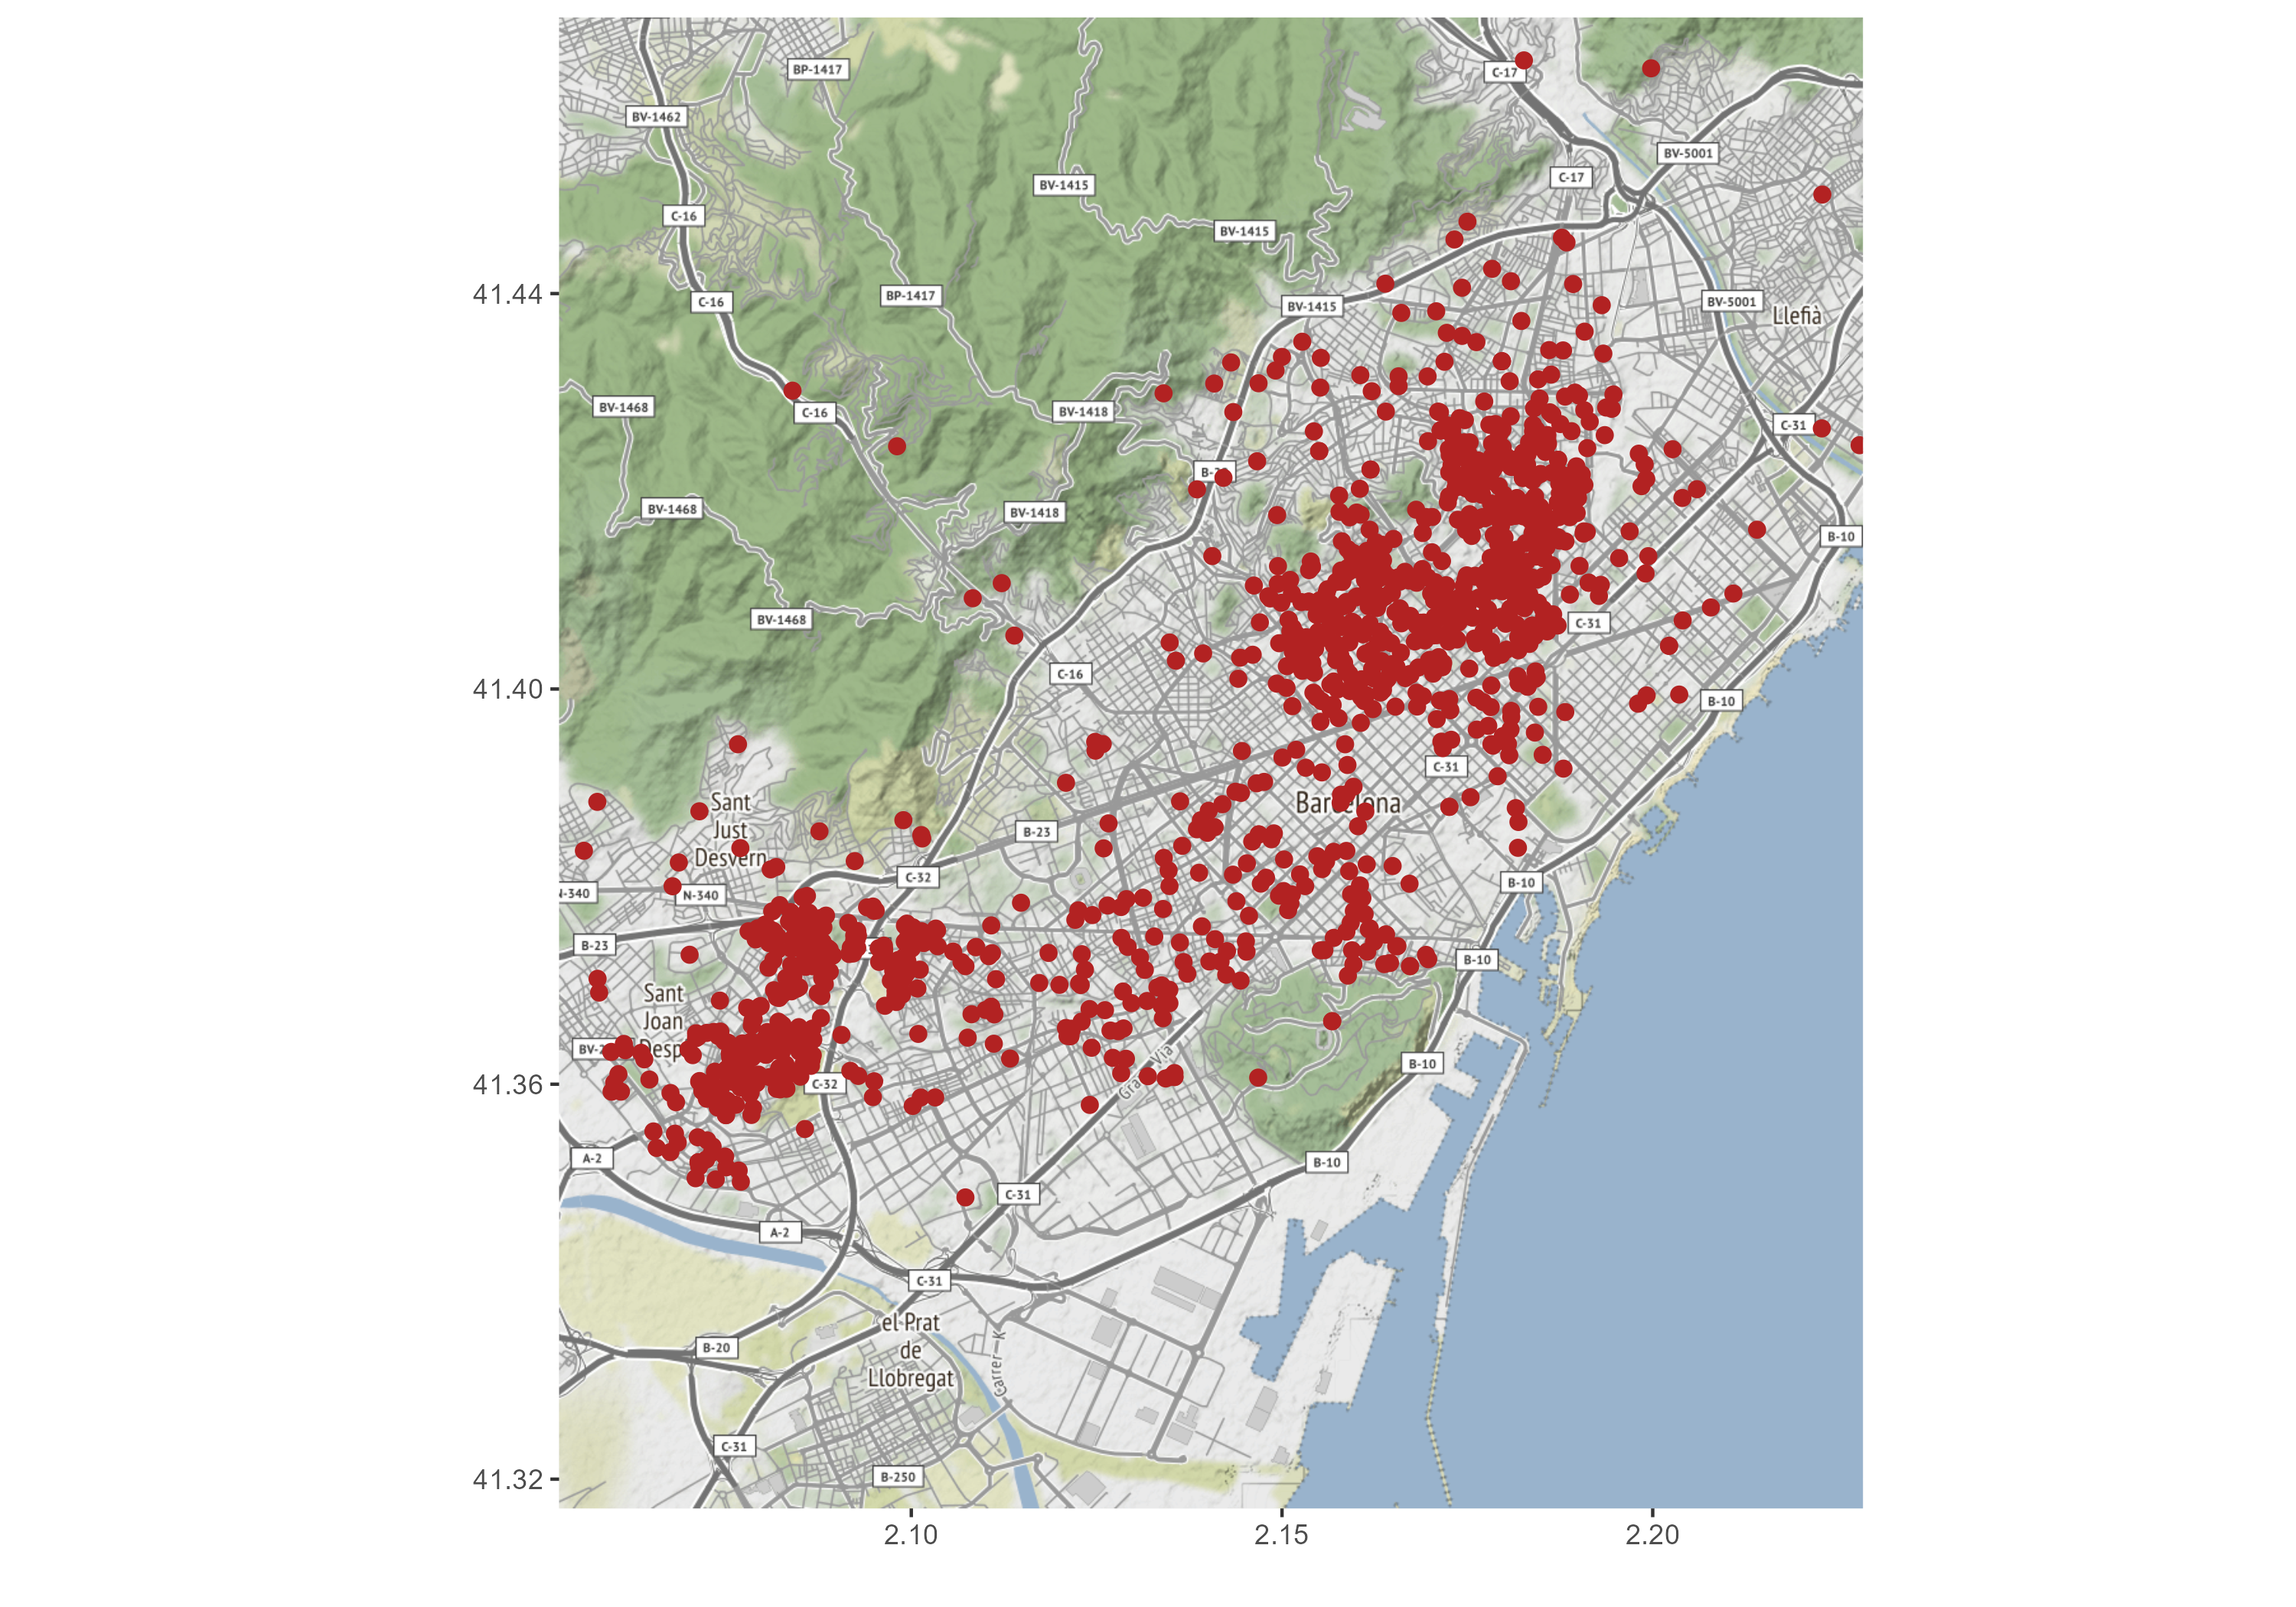
\includegraphics[width=1\textwidth]{figures/bcn_map.png}
\caption{ Study domain and spatial distribution of the BiSC participants (n = 1,083)}
\label{fig1}
\end{figure}

Air pollution measurements were conducted during two separated monitoring campaigns. The first campaign was carried out in accordance with the ESCAPE guidelines. This included four distinct measurements periods: three in the winter, summer, and autumn of 2021, and a final one in the winter of 2022. During these periods, levels of NO\textsubscript{2}, PM\textsubscript{2.5}, and BC were measured at 34 locations across Barcelona Metropolitan Area (Barcelona, Esplugues de Llobregat, and L'Hospitalet). This monitoring campaign was named "BiSCAPE" campaign. The second monitoring campaign was conducted at homes of the BiSC participants, one week during the first trimester and one week during the third trimester of pregnancy, during the period 2018-2021, and only NO\textsubscript{2} levels were measured. This monitoring campaign was named "BiSC-Home" campaign. These monitoring campaigns where used in the development of the LUR and HM models. 

\newpage
%%%%%%%%%%%%%%%%%%%%%%%%%%
%%% --- LUR model --- %%%
%%%%%%%%%%%%%%%%%%%%%%%%%%
\subsection{LUR models}

LUR models for NO\textsubscript{2}  were developed using only data from the locations that had measured home-outdoor (BiSC-Home campaign) levels for both sampling campaigns (i.e., we did not use data from participants who had data available for only one campaign, either first or third trimester). Almost half of the sites were measured before the COVID-19 pandemic started and half of the sites during the pandemic period and its resulting restrictions. For PM\textsubscript{2.5}, PM\textsubscript{2.5} constituents, and BC models were developed using BiSCAPE data from the 34 sites. In addition, for the development of the LUR models, spatial variables that better represent the pollutant concentration distribution across the study area were created. Following the ESCAPE guidelines, we selected predictor variables from three broad categories: traffic, land use, and urban configuration. We selected a wide variety of buffer sizes, i.e, 25m, 50m, 100m, 300m, 500m, and 1000m to capture the area-specific predictor variable at every single location. 

Following the ESCAPE guidelines \cite{eeftens2012, beelen2013}, we applied a supervised stepwise process in which we sequentially add a predictor variable to a linear regression model using pollutant concentrations as the independent variable to obtain the best possible model. This procedure was followed to built all the specific pollutant models. Previously to model development, we specified the direction expected of the effect that each predictor have in the model. 




%%%%%%%%%%%%%%%%%%%%%%%%%%%%%%%%%
%%% --- Dispersion model --- %%%
%%%%%%%%%%%%%%%%%%%%%%%%%%%%%%%%
\subsection{Dispersion models}


%%%%%%%%%%%%%%%%%%%%%%%%%%%%%
%%% --- Hybrid model --- %%%
%%%%%%%%%%%%%%%%%%%%%%%%%%%%
\subsection{Hybrid models}






\subsection{Evaluation}
We performed different assessment to evaluate the performance and accuracy of the obtained models. For LUR models 

%%%%%%%%%%%%%%%%%%%%%%%%%%%
%%% --- References --- %%%
%%%%%%%%%%%%%%%%%%%%%%%%%%%

\bibliography{references}


\end{document}